\documentclass[tikz, border=10pt]{standalone}
\usepackage[utf8]{inputenc}
\usepackage[T1]{fontenc}
\usetikzlibrary{shapes, arrows.meta, positioning, calc, shadows, decorations.pathmorphing}

% Define colors from your lecture notes
\definecolor{primaryblue}{RGB}{0,73,135}
\definecolor{accentgold}{RGB}{198,146,20}
\definecolor{darkgray}{RGB}{64,64,64}
\definecolor{lightgray}{RGB}{240,240,240}
\definecolor{quotegreen}{RGB}{34,139,34}
\definecolor{perilred}{RGB}{160, 20, 20}

\begin{document}

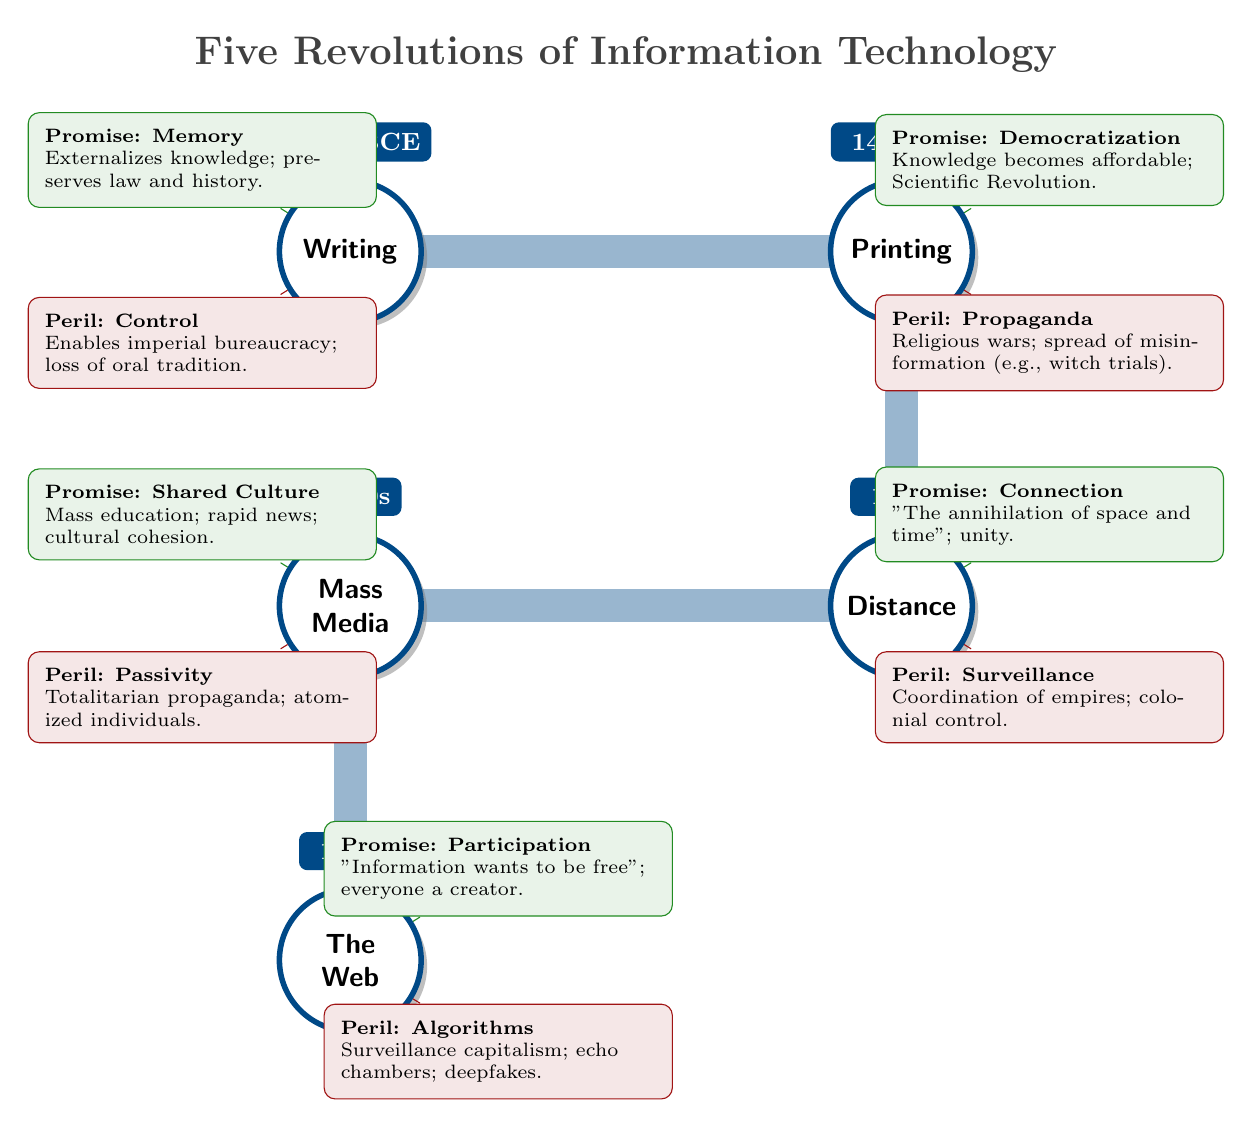
\begin{tikzpicture}[
    % Global Styles
    font=\sffamily,
    scale=1,
    transform shape,
    % Node Styles
    milestone/.style={
        circle, 
        draw=primaryblue, 
        line width=2pt, 
        fill=white, 
        minimum size=1.8cm, 
        align=center, 
        drop shadow
    },
    yearlabel/.style={
        fill=primaryblue, 
        text=white, 
        rounded corners=3pt, 
        font=\bfseries\small, 
        inner sep=4pt
    },
    promisebox/.style={
        rectangle, 
        draw=quotegreen, 
        fill=quotegreen!10, 
        rounded corners, 
        text width=4cm, 
        align=left, 
        inner sep=6pt, 
        font=\scriptsize
    },
    perilbox/.style={
        rectangle, 
        draw=perilred, 
        fill=perilred!10, 
        rounded corners, 
        text width=4cm, 
        align=left, 
        inner sep=6pt, 
        font=\scriptsize
    },
    connector/.style={
        primaryblue!40, 
        line width=12pt, 
        rounded corners=20pt
    },
    arrowhead/.style={
        -{Triangle[width=12pt,length=8pt]}, 
        primaryblue!40, 
        line width=12pt
    }
]

    % --- The Winding Path ---
    % We define coordinates first to draw the path "behind" the nodes
    \coordinate (c1) at (0, 0);
    \coordinate (c2) at (7, 0);
    \coordinate (c3) at (7, -4.5);
    \coordinate (c4) at (0, -4.5);
    \coordinate (c5) at (0, -9);

    % Draw the connecting lines
    \draw[connector] (c1) -- (c2);
    \draw[connector] (c2) -- (c3);
    \draw[connector] (c3) -- (c4);
    \draw[arrowhead] (c4) -- (c5);

    % --- Milestone 1: Writing ---
    \node[milestone] (m1) at (c1) {\textbf{Writing}};
    \node[yearlabel, above=0.2cm of m1] {~3200 BCE};
    
    \node[promisebox, above left=0.5cm and -1cm of m1, anchor=east] (p1a) {
        \textbf{Promise: Memory}\\
        Externalizes knowledge; preserves law and history.
    };
    \node[perilbox, below left=0.5cm and -1cm of m1, anchor=east] (p1b) {
        \textbf{Peril: Control}\\
        Enables imperial bureaucracy; loss of oral tradition.
    };
    \draw[dashed, quotegreen] (m1) -- (p1a);
    \draw[dashed, perilred] (m1) -- (p1b);

    % --- Milestone 2: Printing ---
    \node[milestone] (m2) at (c2) {\textbf{Printing}};
    \node[yearlabel, above=0.2cm of m2] {~1440 CE};
    
    \node[promisebox, above right=0.5cm and -1cm of m2, anchor=west] (p2a) {
        \textbf{Promise: Democratization}\\
        Knowledge becomes affordable; Scientific Revolution.
    };
    \node[perilbox, below right=0.5cm and -1cm of m2, anchor=west] (p2b) {
        \textbf{Peril: Propaganda}\\
        Religious wars; spread of misinformation (e.g., witch trials).
    };
    \draw[dashed, quotegreen] (m2) -- (p2a);
    \draw[dashed, perilred] (m2) -- (p2b);

    % --- Milestone 3: Distance ---
    \node[milestone] (m3) at (c3) {\textbf{Distance}};
    \node[yearlabel, above=0.2cm of m3] {~1840s};
    
    \node[promisebox, above right=0.5cm and -1cm of m3, anchor=west] (p3a) {
        \textbf{Promise: Connection}\\
        "The annihilation of space and time"; unity.
    };
    \node[perilbox, below right=0.5cm and -1cm of m3, anchor=west] (p3b) {
        \textbf{Peril: Surveillance}\\
        Coordination of empires; colonial control.
    };
    \draw[dashed, quotegreen] (m3) -- (p3a);
    \draw[dashed, perilred] (m3) -- (p3b);

    % --- Milestone 4: Mass Media ---
    \node[milestone] (m4) at (c4) {\textbf{Mass}\\\textbf{Media}};
    \node[yearlabel, above=0.2cm of m4] {~1920s};
    
    \node[promisebox, above left=0.5cm and -1cm of m4, anchor=east] (p4a) {
        \textbf{Promise: Shared Culture}\\
        Mass education; rapid news; cultural cohesion.
    };
    \node[perilbox, below left=0.5cm and -1cm of m4, anchor=east] (p4b) {
        \textbf{Peril: Passivity}\\
        Totalitarian propaganda; atomized individuals.
    };
    \draw[dashed, quotegreen] (m4) -- (p4a);
    \draw[dashed, perilred] (m4) -- (p4b);

    % --- Milestone 5: The Web ---
    \node[milestone] (m5) at (c5) {\textbf{The}\\\textbf{Web}};
    \node[yearlabel, above=0.2cm of m5] {~1990s};
    
    \node[promisebox, above right=0.5cm and -1cm of m5, anchor=west] (p5a) {
        \textbf{Promise: Participation}\\
        "Information wants to be free"; everyone a creator.
    };
    \node[perilbox, below right=0.5cm and -1cm of m5, anchor=west] (p5b) {
        \textbf{Peril: Algorithms}\\
        Surveillance capitalism; echo chambers; deepfakes.
    };
    \draw[dashed, quotegreen] (m5) -- (p5a);
    \draw[dashed, perilred] (m5) -- (p5b);
    
    % --- Title Node ---
    \node[align=center, font=\Large\bfseries, text=darkgray] at (3.5, 2.5) {Five Revolutions of Information Technology};

\end{tikzpicture}

\end{document}